% !TEX encoding = UTF-8 Unicode
%!TEX root = thesis.tex
% !TEX spellcheck = en-US
%%=========================================
\section{Experiment 5}
In this experiment, we do 5 fx in parallel => ok result
am
bandpass
bitreduce
dist lpf
chorus

(Then 2 layers of 5?)
Then 10 fx in parallel => bad result

Suggest pre-training with each fx separately, then training the mix
Softmax mixing may also be bad -> suggest independent mix values

create video demonstrating 1st successful result here

Say something about hypothesis about which fx will be used. Which ones were actually used? Do the same for parameters. Show mix values in horizon graph. Say that am and chorus make sound richer, while we need it filtered.

\begin{figure}[h]
    \centering
    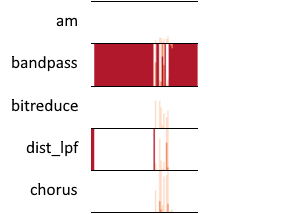
\includegraphics[width=0.3\textwidth]{exp5_1layer_softmax}
    \caption{TODO caption}
    \label{fig:exp5_1layer_softmax}
\end{figure}

\begin{figure}[h]
    \centering
    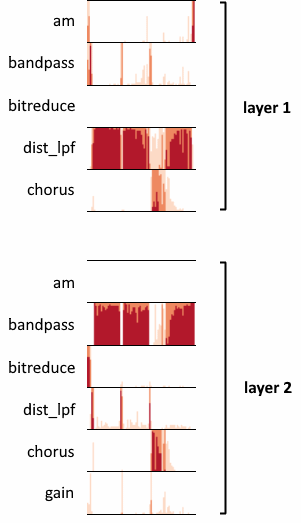
\includegraphics[width=0.45\textwidth]{exp5_2layers_softmax}
    \caption{TODO caption}
    \label{fig:exp5_2layers_softmax}
\end{figure}

\begin{figure}[h]
    \centering
    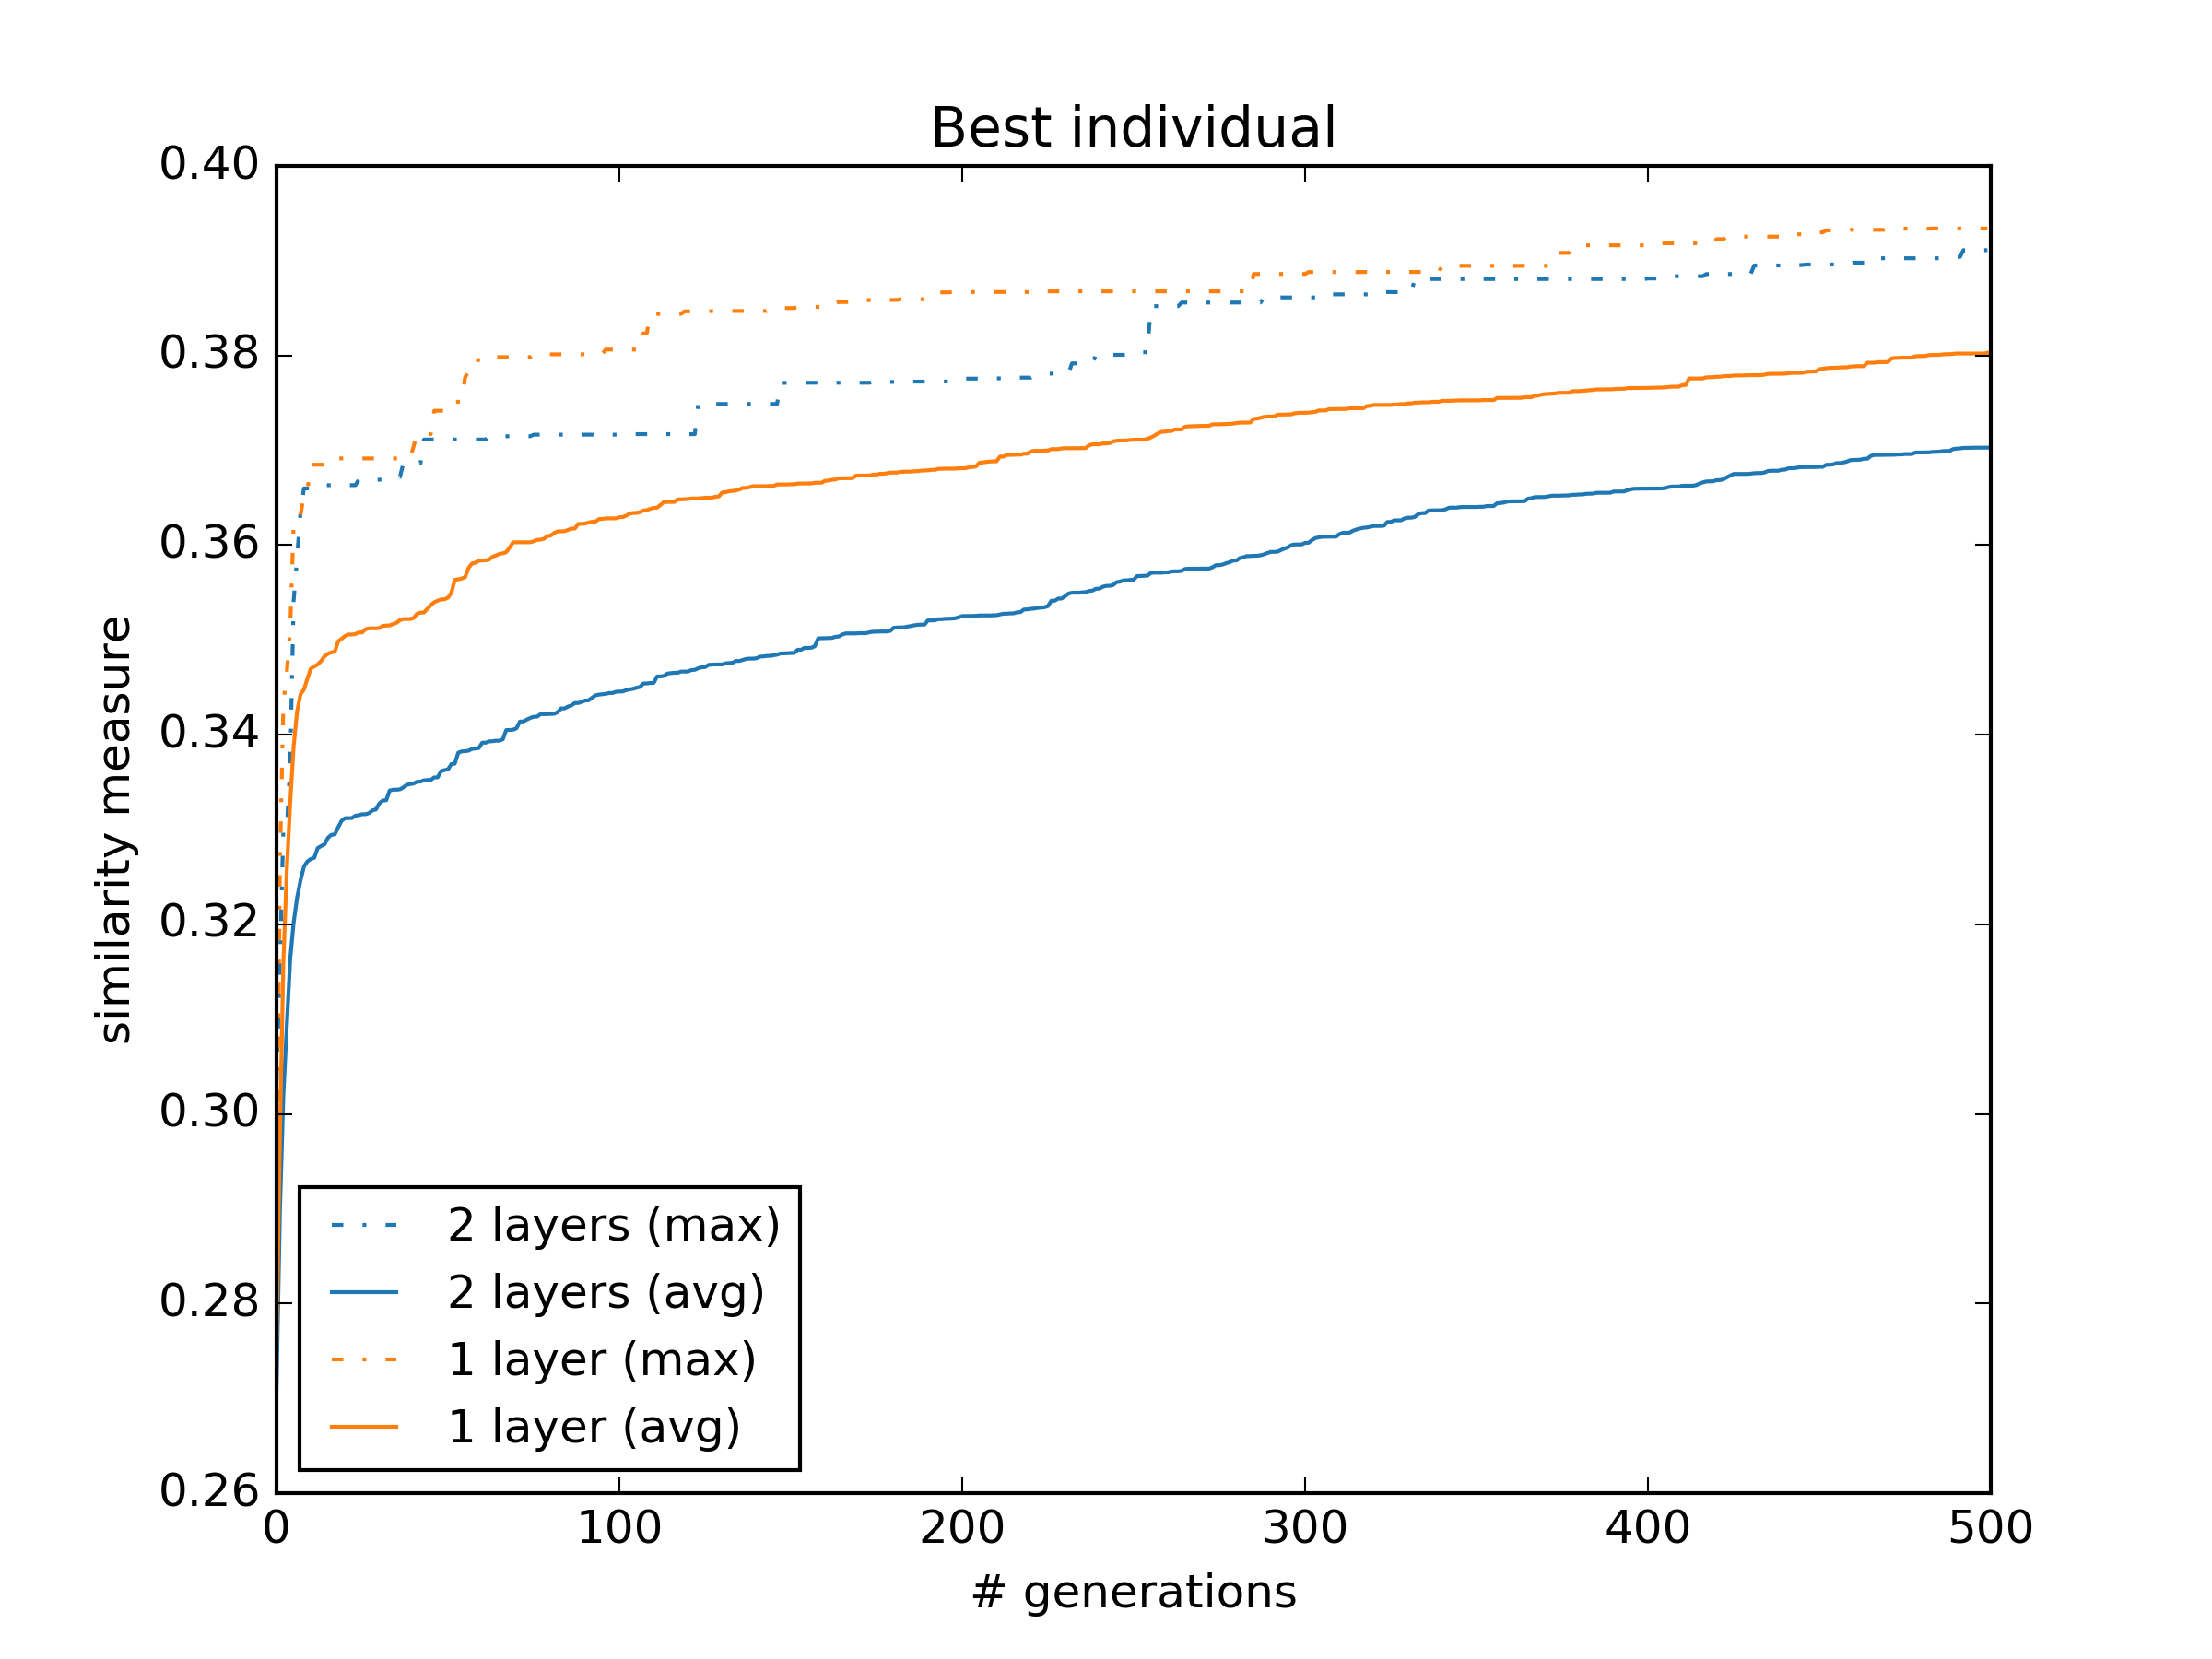
\includegraphics[width=0.99\textwidth]{exp5_avg_max}
    \caption{Aggregated fitness values}
    \label{fig:exp5_avg_max}
\end{figure}

\begin{figure}[h]
    \centering
    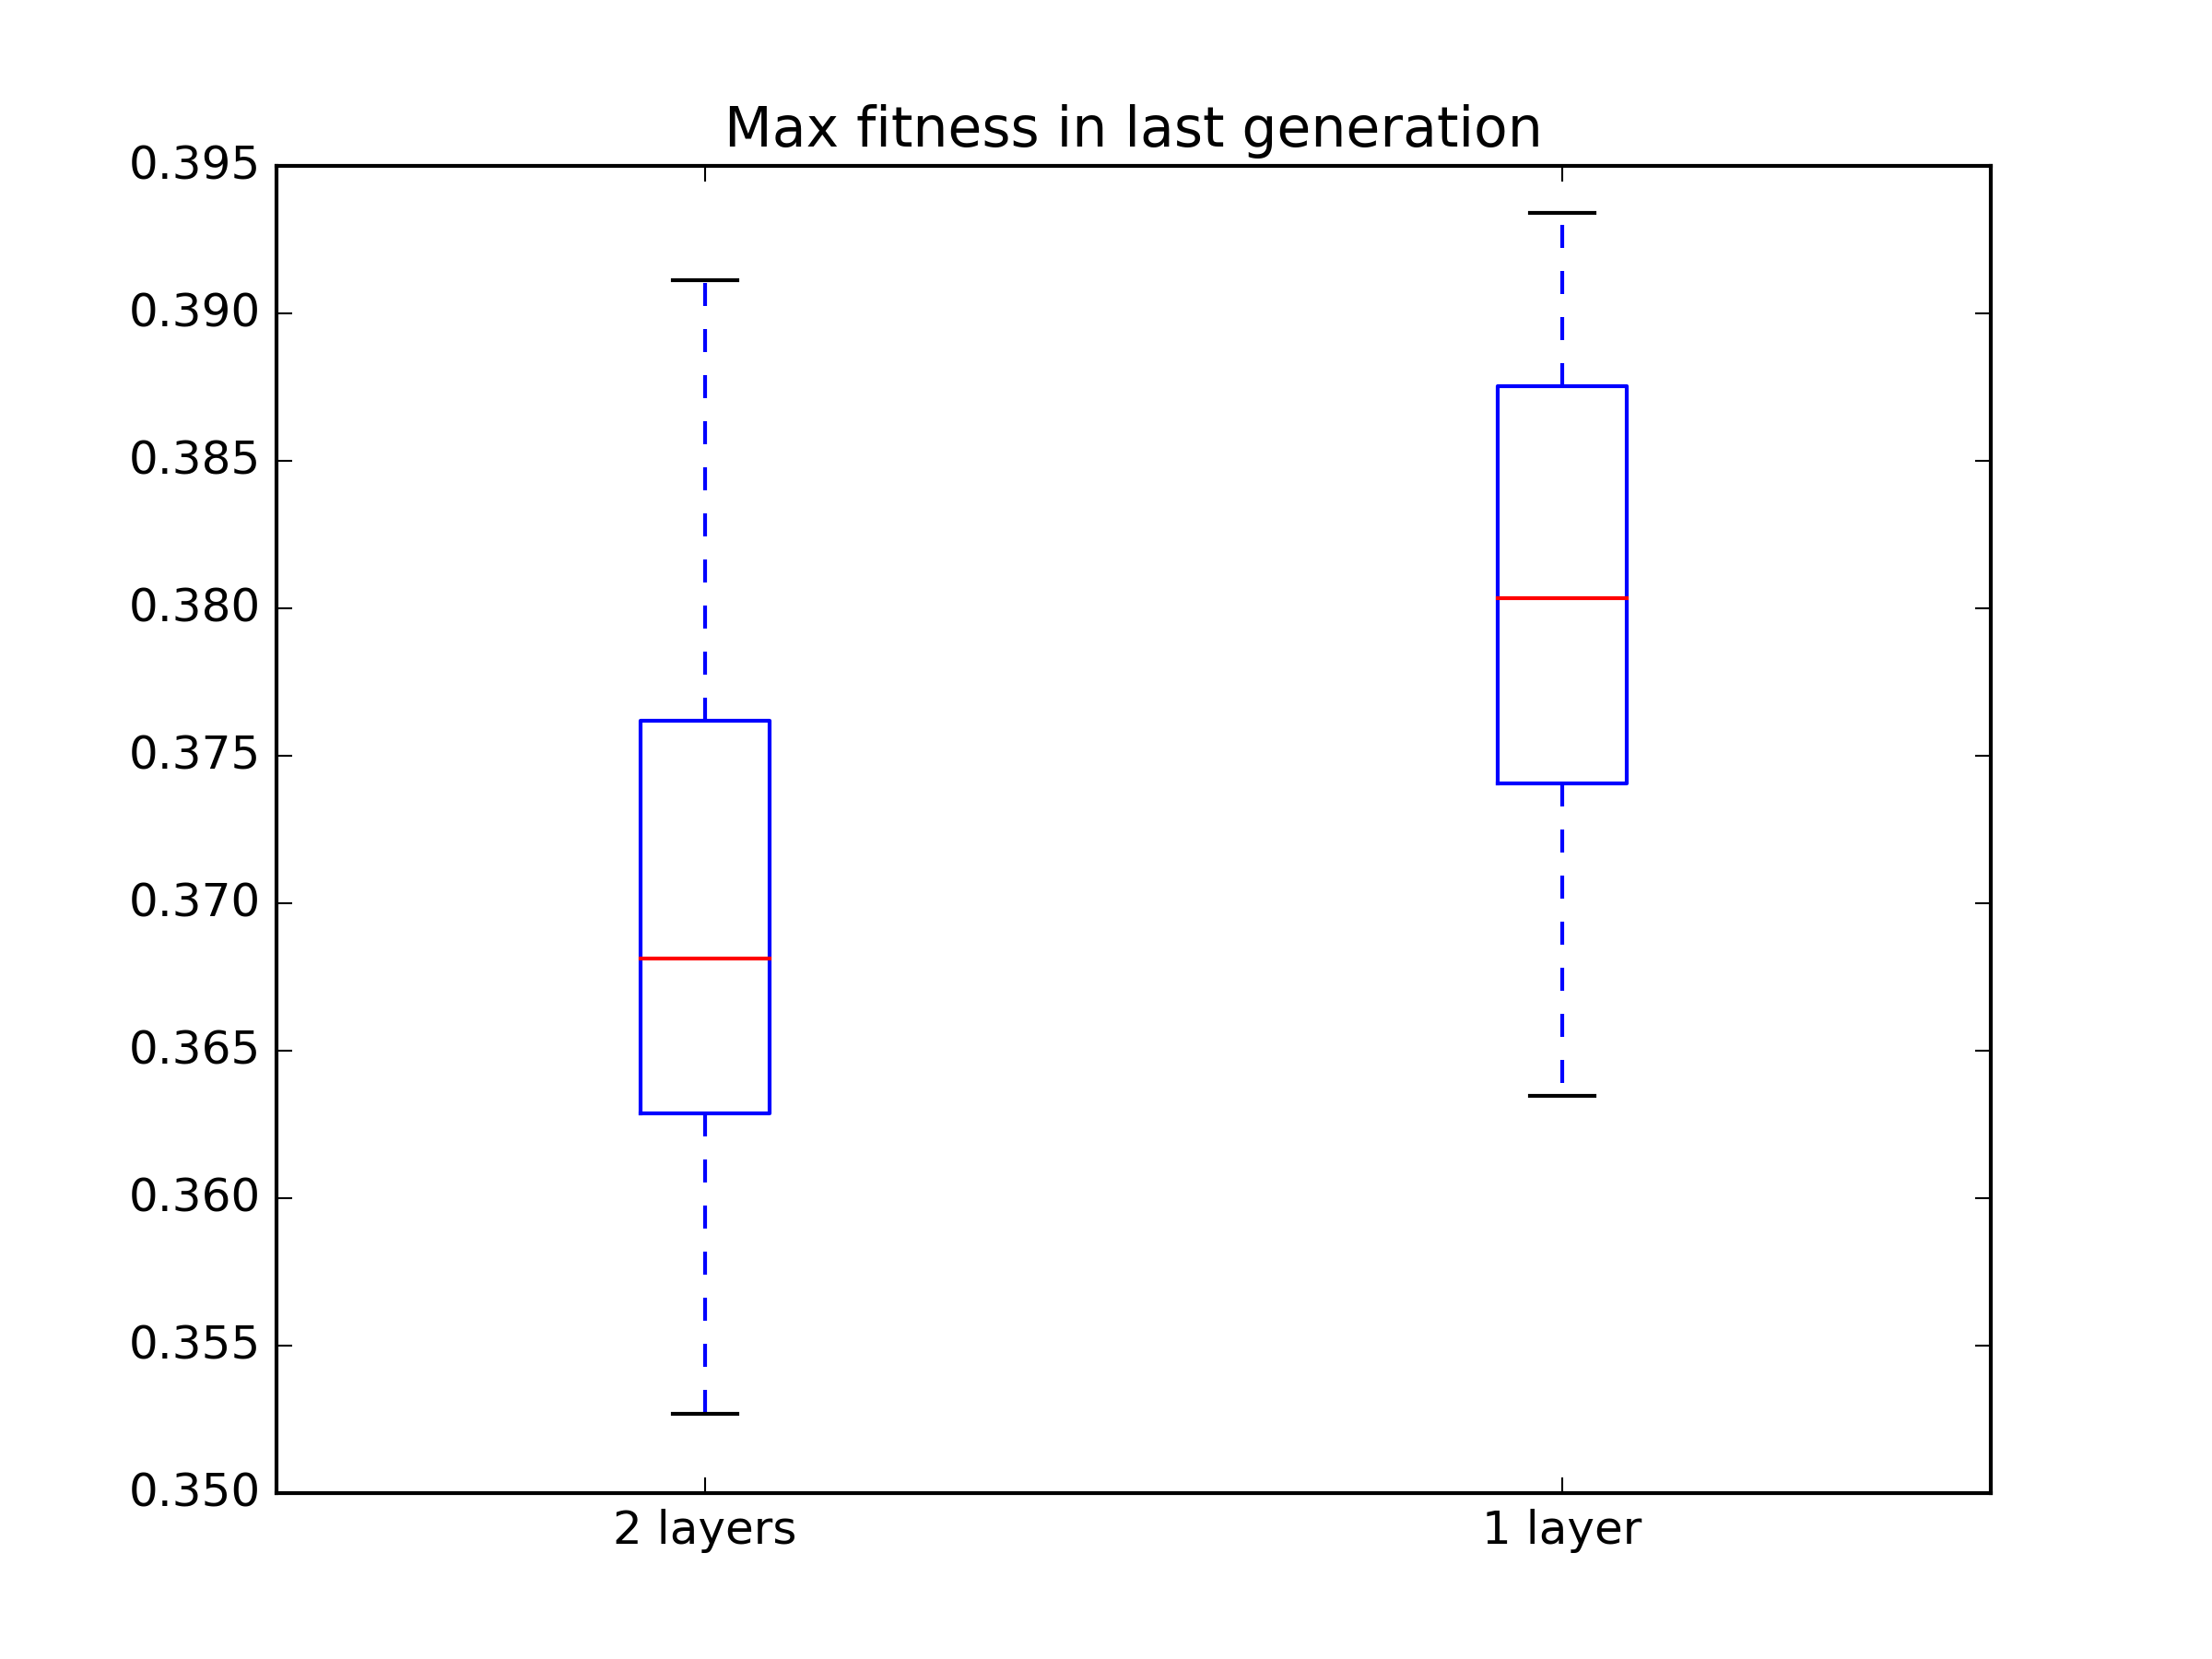
\includegraphics[width=0.99\textwidth]{exp5_box}
    \caption{Box-and-whiskers plot of fitness values in the last generation}
    \label{fig:exp5_box}
\end{figure}
